\documentclass[11pt, oneside]{article} 
\usepackage{geometry}
\geometry{letterpaper} 
\usepackage{graphicx}
	
\usepackage{amssymb}
\usepackage{amsmath}
\usepackage{parskip}
\usepackage{color}
\usepackage{hyperref}

\graphicspath{{/Users/telliott/Dropbox/Github-Math/geoproof/figures/}{/Users/telliott/Dropbox/Github-Math/figures/}}
% \begin{center} \includegraphics [scale=0.4] {gauss3.png} \end{center}


\title{Parallel or perpendicular}
\date{}

\begin{document}
\maketitle
\Large

%[my-super-duper-separator]

\subsection*{right angles}

When two lines cross, they form four angles.

$\circ$ \ If the angles adjacent to each other (on one side of any line) are equal, then we say that those angles are both right angles.  

For a Greek mathematician, this is the definition of a right angle.  If adjacent angles are equal, both are right angles. They also had an axiom about them:  that \emph{all right angles are equal}.

We say that two lines which cross to form right angles are \emph{perpendicular}.
\begin{center} 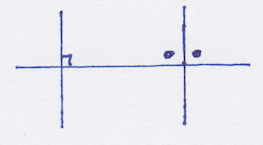
\includegraphics [scale=0.7] {B4.png} \end{center}

I'm sure you've been taught that the \emph{measure} of a right angle is $90^{\circ}$.  But the Greeks never used degrees. We will write $180$ when we mean two right angles, and perhaps, 90 when we mean one, only because it is more concise.

In the figure above, on the left, a standard symbol for a right angle is shown:  a small square.  On the right, we have marked two equal angles with dots.  This is much cleaner than the standard notation, which uses arcs and bars.  It's even better when you can use colored circles.

When one of the four angles formed by two lines crossing is a right angle, all four of them are right angles.  

Each angle above is adjacent to two different angles, so both of those are equal right angles.  And in turn they are both adjacent to the fourth angle, so it is a right angle as well.

\subsection*{parallel lines}
$\circ$ \ If two lines are drawn so that they never cross, they are parallel lines.

Arrowheads indicate that a line continues in both directions, forever.
\begin{center} 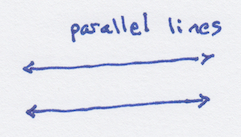
\includegraphics [scale=0.7] {B7.png} \end{center}

Parallel lines never meet.  They are the same distance apart, everywhere along their lengths.

This leads to the question of how to measure the distance between two lines.  That's actually a tricky question so we will not try to answer it now.  

Let's just say that we choose a point on one line, then measure the distance to the second line along a perpendicular from the first.  Move the first point over a bit and repeat the measurement.  If it changes, the two lines are not parallel.

Suppose the second line is 1 foot from the first at given point, but further along in a particular direction, say 1 mile, we measure 11 inches instead.  

Why would this be problem?  Since a line goes forever, if we travel 12 miles that down the road rather than one, the two lines that we supposed were parallel, would meet.  We must conclude that they are not parallel after all.

$\circ$ \ Two parallel lines never meet and they stay exactly the same distance apart, forever.

We can make a similar statement about line segments.  Here $L1 \parallel L2$ and $AB \parallel CD$.
\begin{center} 
\includegraphics [scale=0.7] {B7b.png} 
\includegraphics [scale=0.7] {B8b.png} 
\end{center}
We mean that, if both line segments were extended to be lines, they would never cross.

An open circle ($\circ$), is used to mark an important statement, an assumption or \emph{axiom} about the world.  We will need a few of those, to get started.  

We also assume \emph{common notions}, such as that equals added to equals are equal, and that a thing is equal to itself.  We gladly accept these as well, without much fanfare.

Other statements are  \emph{theorems}, marked with a $\bullet$, truths that we have deduced in a particular situation shown by a diagram.  In the next chapter we get started on proving theorems.  We will not stop until the end.

\end{document}
